% Use LuaLaTeX to compile
\documentclass[aspectratio=169]{beamer}
\usetheme{metropolis}
\metroset{sectionpage=none}
\metroset{progressbar=frametitle}
\metroset{block=fill}

% Declare environment blockitem
\newenvironment{blockitem}[1]{\begin{block}{#1}\begin{itemize}}{\end{itemize}\end{block}}
\newenvironment{blockenum}[1]{\begin{block}{#1}\begin{enumerate}}{\end{enumerate}\end{block}}

% Macro for fragile frames
\newenvironment{xframe}[1][]%
	{\begin{frame}[fragile, environment=xframe, #1]{\secname}}%
	{\end{frame}}

% Declare command TODO: text in red
\newcommand{\todo}[1]{\textcolor{red}{TODO: #1}}

\usepackage{tikz}
\usetikzlibrary{shapes,arrows}
\usetikzlibrary{arrows.meta}
\usetikzlibrary{decorations.pathreplacing}
\usetikzlibrary{positioning,shapes.geometric}
\usetikzlibrary{
arrows,
decorations.pathreplacing,
graphs,
graphs.standard,
patterns,
positioning,
shapes.geometric
}

\usepackage{graphicx}
\usepackage[mode=buildnew]{standalone}
\usepackage{pdfpages}

\usepackage{tabularx}
\usepackage{booktabs}

\usepackage{xspace}

\usepackage{adjustbox}

\usepackage{ourmacros-private}

\usepackage{pgfplots}

\usepackage{adjustbox}

\usepackage{caption}

\usepackage{multirow}
\usepackage{booktabs}
\usepackage{color, colortbl}
\definecolor{lgreen}{rgb}{0.7, 1, 0.7}
\definecolor{lred}{rgb}{1, 0.7, 0.7}
\definecolor{lyellow}{rgb}{1, 1, 0.7}

\usepackage{mdframed}

\usepackage{minted}
\setminted{fontsize=\scriptsize, breaklines=true, breakanywhere=true, breakautoindent=true, breakafter={.,}, breakaftersymbolpre={\ }, breakaftersymbolpost={\ },
	escapeinside=||,
	autogobble=true,
	linenos=false,
	tabsize=2,
	% frame=lines,
	% framesep=2mm,
	% rulecolor=\color{black!30},
	% bgcolor=gray!5,
}
\BeforeBeginEnvironment{minted}{\begin{mdframed}}
\AfterEndEnvironment{minted}{\end{mdframed}}

\usepackage{newverbs}
\newverbcommand{\cverb}{\color{blue}}{}

\newcommand{\colorref}[3][blue]{\href{#2}{\texttt{\textcolor{#1}{#3}}}}

\usepackage{siunitx}
\sisetup{per-mode=symbol}
\DeclareSIUnit{\FLOP}{FLOP}
\DeclareSIUnit{\empty}{{}}

\usepackage[%
	backend=biber,
	style=verbose,
	autocite=footnote,
	]
	{biblatex}
\addbibresource{references.bib}

\title{What You Always Wanted To Know About \langcpp Performance Portability (But Were Afraid to Do)}
\subtitle{Austrian-Slovenian HPC Meeting 2024 --- ASHPC24}
\date{June 12, 2024}
\author{%
	Ruben Laso, Diego Krupitza, and Sascha Hunold \\
	\texttt{\{\href{mailto:laso@par.tuwien.ac.at}{laso}, \href{mailto:krupitza@par.tuwien.ac.at}{krupitza}, \href{mailto:hunold@par.tuwien.ac.at}{hunold}\}@par.tuwien.ac.at}
}
\institute{Research Group for Parallel Computing, TU Wien}

\begin{document}

% Insert TU Wien and research group logos in the title slide
% \titlegraphic{
% 	\vspace{-10pt}
% 	
\includegraphics[height=20pt]{images/Par_logo}
% 	\hspace{5pt}
% 	
\includegraphics[height=20pt]{images/TU_Logo}
% }

% \maketitle

\begin{frame}
	\titlepage
	\begin{tikzpicture}[overlay, remember picture]
		\node[above right=.5cm and .8cm of current page.south west] {
\includegraphics[height=20pt,clip]{images/Par_logo.pdf}};
		\node[above right=.5cm and 1.8cm of current page.south west] {
\includegraphics[height=20pt]{images/TU_Logo.pdf}};
	\end{tikzpicture}
\end{frame}


\section*{\langcpp STL in HPC}
\begin{xframe}
	\begin{blockitem}{\langcpp in High-Performance Computing}
		\item Languages like C, \langcpp and Fortran are the most used in HPC
		\begin{itemize}
			\item Existing code base
			\item Performance
			\item Compatibility with new hardware
		\end{itemize}
		\item \langcpp can be used in several types of architectures
		\begin{itemize}
			\item Multi-core and many-core CPUs $\rightarrow$ OpenMP, TBB
			\item GPUs $\rightarrow$ CUDA, OpenCL
			\item FPGAs $\rightarrow$ SYCL
		\end{itemize}
		\item Should we use a different code for each system?
	\end{blockitem}
\end{xframe}

\begin{xframe}
	\begin{block}{Performance Portability}
		Same code performs ``well'' on different architectures
	\end{block}
	\begin{blockitem}{Performance Portability in \langcpp}
		\item Several libraries: Kokkos, RAJA, HPX, \dots
		\item \textbf{\langcppsvtn} with \textbf{execution policies}
		\begin{itemize}
			\item Parallel execution of the algorithms in STL (standard library)
			\item Different compilers/backends
		\end{itemize}
	\end{blockitem}
\end{xframe}

\begin{xframe}
	\begin{blockitem}{Questions}
		\item \textbf{Speedup and efficiency} of parallel STL algorithms?
		\item Which is the \textbf{best compiler/backend}? GCC vs ICC, TBB vs OpenMP, \dots
		\item \textbf{GPUs} performance?
	\end{blockitem}
	\begin{blockitem}{Contributions}
		\item \pstlbench: micro-benchmark suite
		\item Evaluation of the performance for
		\begin{itemize}
			\item Different compilers: GCC, ICC, NVIDIA HPC SDK
			\item Different backends: OpenMP, TBB, HPX, CUDA
			\item Different systems: Intel and AMD CPUs, NVIDIA GPUs
		\end{itemize}
	\end{blockitem}
\end{xframe}

\section*{pSTL-Bench}

\begin{xframe}
	\begin{blockitem}{pSTL-Bench}
		\item Code available on \colorref{https://github.com/parlab-tuwien/pSTL-Bench}{github.com/parlab-tuwien/pSTL-Bench}
		\item Suite of \textbf{micro-benchmarks} to test performance portability in \langcpp
		\begin{itemize}
			\item STL algorithms: \verb|std::for_each|, \verb|std::reduce|, \verb|std::sort|, \dots
		\end{itemize}
		\item Features:
		\begin{itemize}
			\item Number of threads: with \verb|OMP_NUM_THREADS| or \verb|--hpx::threads=N|
			\item HW Perf. Counters: PAPI's HL or Likwid's Marker APIs
			\item Different (customizable) input sizes and data types
			\item Custom NUMA allocator
		\end{itemize}
	\end{blockitem}
\end{xframe}

\section*{Experiments}

\begin{xframe}
	\begin{blockitem}{Variables}
		\item Input sizes: $2^{3}$ to $2^{30}$ elements $\rightarrow$ 64B to 8GB
		\item Data type: \verb|double| and \verb|float|
		\item \pstlbench's NUMA allocator
		\item No control of thread and memory placement
	\end{blockitem}
	\begin{blockitem}{Contenders}
		\item Compilers: GCC, ICC, NVIDIA HPC SDK
		\item Backends: GNU (OpenMP), TBB, HPX, Thrust (OMP), CUDA
	\end{blockitem}
\end{xframe}

\begin{xframe}
	\setlength{\tabcolsep}{4pt}
\begin{center}
	\begin{adjustbox}{max width=\textwidth, max height=\textheight}
		\begin{tabular}{lrrrr}
			\toprule
			Machine                                                 & \machvsclong                    & \machhydralong                  & \machteslalong            & \machamperelong            \\
			\midrule
			CPU/GPU                                                 & \textbf{AMD EPYC 7713}          & \textbf{Intel Xeon 6130F}       & \textbf{\nvidia Tesla T4} & \textbf{\nvidia Ampere A2} \\
			Architecture                                            & Zen 3                           & Skylake                         & Turing                    & Ampere                     \\
			% Core frequency                                          & \qty{2.00}{\giga\hertz}         & \qty{2.10}{\giga\hertz}         & \qty{1.11}{\giga\hertz}  & \qty{1.77}{\giga\hertz}  \\
			Sockets \textbar{} NUMA nodes                           & 2 \textbar{} 8                  & 2 \textbar{} 2                  & 1 \textbar{} 1            & 1 \textbar{} 1             \\
			Total \#cores \textbar{} threads                        & 128 \textbar{} 256              & 32 \textbar{} 32                & 2560 \textbar{} 2560      & 1280 \textbar{} 1280       \\
			Max. \#threads used                                     & \textbf{128}                    & \textbf{32}                     & \textbf{2560}             & \textbf{1280}              \\
			Memory (node / GPU)                                     & \qty{512}{\gibi\byte}           & \qty{48}{\gibi\byte}            & \qty{16}{\gibi\byte}      & \qty{8}{\gibi\byte}        \\
			Memory (per core)                                       & \qty{4}{\gibi\byte}             & \qty{1.5}{\gibi\byte}           & —                         & —                          \\
			% \midrule
			% Compilers                                               & \gppvsc                         & \gpphydra                       & \gpptesla                & \gppampere               \\
			%                                                         & \nvhpcvsc                       & \nvhpchydra                     & \nvhpctesla              & \nvhpcampere             \\
			%                                                         & \icpxvsc                        & \icpxhydra                      &                          &                          \\
			% \midrule
			% Libraries                                               & \tbbvsc                         & \tbbhydra                       & \cudatesla               & \cudaampere              \\
			%                                                         & \hpxvsc                         & \hpxhydra                       &                          &                          \\
			%                                                         & \gompvsc                        & \gomphydra                      &                          &                          \\
			%                                                         & \nvompvsc                       & \nvomphydra                     &                          &                          \\
			\midrule
			STREAM BW                                               & \num{42.6} \textbar{} \num{249} & \num{11.7} \textbar{} \num{135} & N/A \textbar{} \num{264}  & N/A \textbar{} \num{172}   \\
			1 \textbar{} all~core(s) (\unit{\giga\byte\per\second}) &                                 &                                 &                           &                            \\
			\bottomrule
		\end{tabular}
	\end{adjustbox}
\end{center}
\end{xframe}

\section*{Results}

\begin{frame}{Results - Execution time scaling}
	\begin{figure}
		\begin{columns}
			\column{0.5\textwidth}
			\includestandalone[width=\textwidth]{charts/vsc/for_each_it1/for_each_problem_size}
			\column{0.5\textwidth}
			\includestandalone[width=\textwidth]{charts/vsc/for_each_it1000/for_each_problem_size}
		\end{columns}
		\caption*{\textbf{Execution time scaling} of \texttt{for\_each} in \machvsclong. Data type: \texttt{double}. \textbf{All cores} are used except for GCC-SEQ. Lower is better.}
	\end{figure}
\end{frame}

\begin{frame}{Results - Speedup}
	\begin{figure}
		\begin{columns}
			\column{0.5\textwidth}
			\includestandalone[width=\textwidth]{charts/vsc/for_each_it1/for_each_speedup}
			\column{0.5\textwidth}
			\includestandalone[width=\textwidth]{charts/vsc/for_each_it1000/for_each_speedup}
		\end{columns}
		\caption*{\textbf{Strong scaling} of \texttt{for\_each} with $2^{30}$ \texttt{double}s in \machvsclong. Higher is better.}
	\end{figure}
\end{frame}

\begin{frame}{Results - GPUs}
	\begin{figure}
		\begin{columns}
			\column{0.5\textwidth}
			\includestandalone[width=\textwidth]{charts/hydra-gpus/reduce/reduce_problem_size_transfer}
			\column{0.5\textwidth}
			\includestandalone[width=\textwidth]{charts/hydra-gpus/reduce/reduce_problem_size_no_transfer}
		\end{columns}
		\caption*{\textbf{Execution time scaling} of \texttt{reduce}. Data type: \texttt{float}. \textbf{All cores} are used except for GCC-SEQ. Lower is better.}
	\end{figure}
\end{frame}

\section*{Get your hands on it}

\begin{xframe}
	\begin{columns}[t]
		\column{0.55\textwidth}
		\begin{blockitem}{Code and papers}
			\small
			\item \pstlbench: \colorref{https://github.com/parlab-tuwien/pSTL-Bench}{github.com/parlab-tuwien/pSTL-Bench}
			\item arXiv preprint: \colorref{https://arxiv.org/abs/2402.06384}{https://arxiv.org/abs/2402.06384}
			\item ICPP 2024 paper: incoming
		\end{blockitem}
		\column{0.45\textwidth}
		\par{}
		\fbox{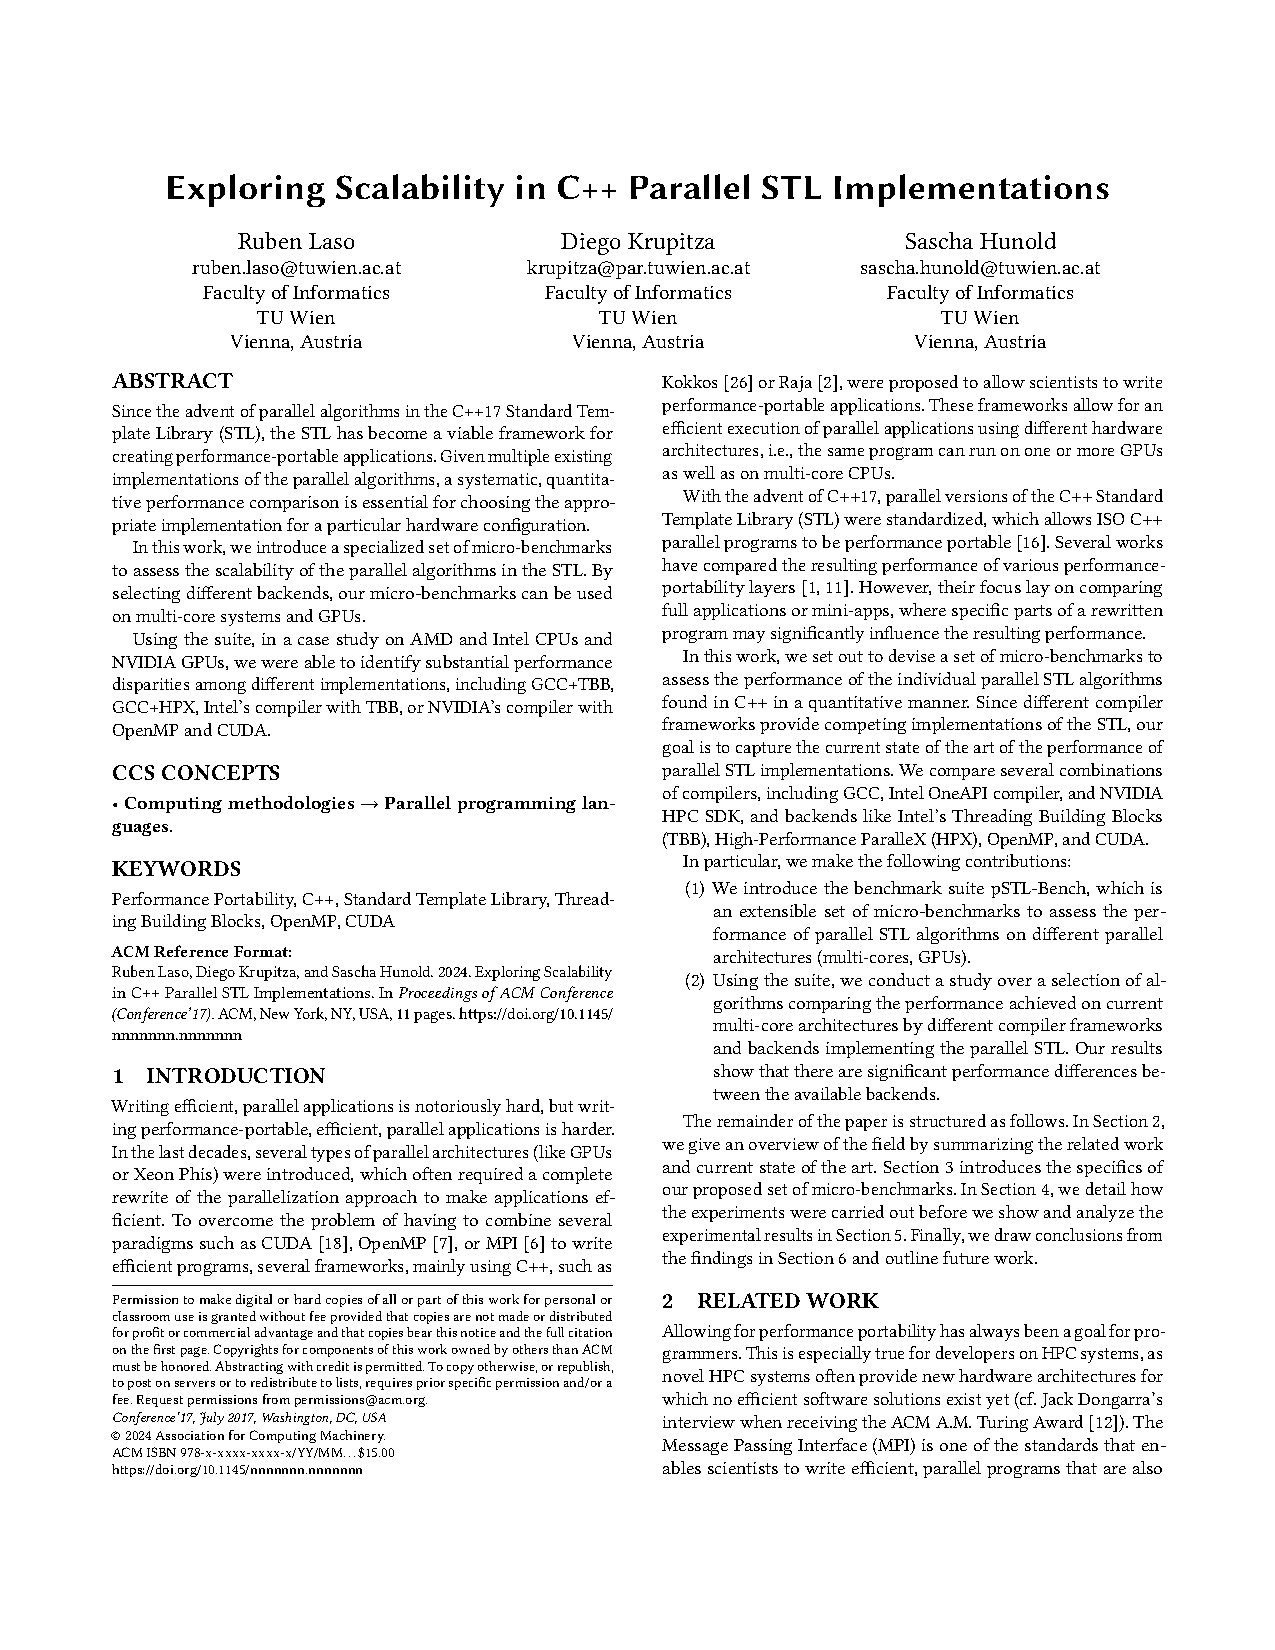
\includegraphics[page=1, width=0.85\textwidth, trim=40 50 40 50]{images/pstl_bench_main.pdf}}
	\end{columns}
\end{xframe}

% Show again the cover title
% \maketitle

\begin{frame}
	\titlepage
	\begin{tikzpicture}[overlay, remember picture]
		\node[above right=.5cm and .8cm of current page.south west] {
\includegraphics[height=20pt,clip]{images/Par_logo.pdf}};
		\node[above right=.5cm and 1.8cm of current page.south west] {
\includegraphics[height=20pt]{images/TU_Logo.pdf}};
	\end{tikzpicture}
\end{frame}


\section*{Additional content}


\begin{xframe}
	% \begin{table}[t]
% 	\caption*{Maximum number of threads such that efficiency is above \qty{70}{\percent} (compared to the seq. execution) for machines \machhydralong, \machnebulalong, and \machvsclong. Notation is \machhydra|\machnebula|\machvsc.  Problem size is $2^{30}$. \higherisbetter.}
% 	\label{tab:threads-with-good-efficiency}
% 	\begin{adjustbox}{max width=\textwidth}
% 	\begin{tabular}{ccccccc}
% 		\toprule
% 		        & \groupfind  & \groupforeach        & \groupforeach          & \groupinclscan  & \groupreduce & \groupsort   \\
% 		        &             & $k_\text{it} = 1 $ & $k_\text{it} = 1000$ &                 &              &              \\
% 		\midrule
% 		GCC-TBB & 2 | 1 | 2   & 8 | 4 | 1            & 32 | 64 | 128          & 4 | 1 | 1       & 32 | 8 | 16  & 8 | 8 | 8    \\
% 		GCC-GNU & 8 | 1 | 1   & 1 | 1 | 1            & 32 | 64 | 128          & N/A | N/A | N/A & 32 | 8 | 16  & 32 | 16 | 32 \\
% 		GCC-HPX & 16 | 4 | 1  & 16 | 2 | 2           & 32 | 32 | 16           & 4 | 2 | 1       & 8 | 2 | 4    & 4 | 2 | 4    \\
% 		ICC-TBB & 2 | N/A | 1 & 8 | N/A | 4          & 32 | N/A | 128         & 4 | N/A | 1     & 4 | N/A | 1  & 8 | N/A | 8  \\
% 		NVC-OMP & 16 | 4 | 4  & 32 | 32 | 16         & 32 | 64 | 128          & 1 | 1 | 1       & 32 | 16 | 32 & 2 | 2 | 2    \\
% 		\bottomrule
% 	\end{tabular}
% 	\end{adjustbox}
% \end{table}

\begin{table}[t]
	\caption*{Maximum number of threads such that \textbf{efficiency is above \qty{70}{\percent}} (compared to the seq. execution) for \machvsclong. Problem size is $2^{30}$. \higherisbetter.}
	\label{tab:threads-with-good-efficiency}
	\begin{adjustbox}{max width=\textwidth}
		\begin{tabular}{ccccccc}
			\toprule
			        & \groupfind & \groupforeach      & \groupforeach        & \groupinclscan & \groupreduce & \groupsort \\
			        &            & $k_\text{it} = 1 $ & $k_\text{it} = 1000$ &                &              &            \\
			\midrule
			GCC-TBB & 2          & 1                  & 128                  & 1              & 16           & 8          \\
			GCC-GNU & 1          & 1                  & 128                  & N/A            & 16           & 32         \\
			GCC-HPX & 1          & 2                  & 16                   & 1              & 4            & 4          \\
			ICC-TBB & 1          & 4                  & 128                  & 1              & 1            & 8          \\
			NVC-OMP & 4          & 16                 & 128                  & 1              & 32           & 2          \\
			\bottomrule
		\end{tabular}
	\end{adjustbox}
\end{table}
\end{xframe}


\begin{xframe}
	\begin{columns}
		\column{0.5\textwidth}
		\begin{table}[t]
	\centering
	\caption*{Executed instructions in 100 calls to \texttt{std::for\_each} ($k_\text{it} = 1$) on \machhydralong.\vspace{-15pt}}
	\label{tab:foreach-hw-counters}
	\begin{adjustbox}{max width=\linewidth}
	\begin{tabular}{lrrrrr}
		\toprule
		\multirow{2}{*}{Metric}                       & GCC   & GCC   & GCC   & ICC   & NVC   \\
		                                              & TBB   & GNU   & HPX   & TBB   & OMP   \\
		\midrule
		Instructions                                  & 1.72T & 2.41T & 3.83T & 1.55T & 2.24T \\
		FP scalar                                     & 107G  & 107G  & 107G  & 107G  & 107G  \\
		FP 128-bit packed                             & 0     & 0     & 0     & 0     & 0     \\
		FP 256-bit packed                             & 0     & 0     & 0     & 0     & 0     \\
		\unit{\giga\FLOP\per\second}                  & 5.41  & 6.51  & 4.06  & 5.02  & 7.26  \\
		Mem. bandwidth (\unit{\gibi\byte\per\second}) & 107.6 & 116.6 & 75.6  & 104.5 & 119.1 \\
		Mem. data volume (\unit{\gibi\byte})          & 2128  & 1925  & 1850  & 2151  & 1762  \\
		\bottomrule
	\end{tabular}
	\end{adjustbox}
\end{table}

% likwid-perfctr -g MEM_DP -m ./pSTL-Bench_GCC_TBB --benchmark_min_time=100x --benchmark_filter="TBB/.*::for_each/.*/1073741824"

% +-----------------------------------------------+---------+---------------+-------------+-------------+--------------+
% |                     Event                     | Counter |      Sum      |     Min     |     Max     |      Avg     |
% +-----------------------------------------------+---------+---------------+-------------+-------------+--------------+
% |             INSTR_RETIRED_ANY STAT            |  FIXC0  | 1718537770000 | 51248530000 | 56030100000 | 5.370431e+10 |
% |           CPU_CLK_UNHALTED_CORE STAT          |  FIXC1  | 1254981000000 | 38160950000 | 39468760000 |  39218156250 |
% |           CPU_CLK_UNHALTED_REF STAT           |  FIXC2  | 1255205390000 | 38171560000 | 39471610000 | 3.922517e+10 |
% |              PWR_PKG_ENERGY STAT              |   PWR0  |     4469.7700 |           0 |   2349.5210 |     139.6803 |
% |              PWR_DRAM_ENERGY STAT             |   PWR3  |      599.6522 |           0 |    301.2830 |      18.7391 |
% | FP_ARITH_INST_RETIRED_128B_PACKED_DOUBLE STAT |   PMC0  |             0 |           0 |           0 |            0 |
% |    FP_ARITH_INST_RETIRED_SCALAR_DOUBLE STAT   |   PMC1  |  107374274000 |  3201975000 |  3500765000 | 3.355446e+09 |
% | FP_ARITH_INST_RETIRED_256B_PACKED_DOUBLE STAT |   PMC2  |             0 |           0 |           0 |            0 |
% | FP_ARITH_INST_RETIRED_512B_PACKED_DOUBLE STAT |   PMC3  |             0 |           0 |           0 |            0 |
% |               CAS_COUNT_RD STAT               | MBOX0C0 |    2243323000 |           0 |  1135304000 | 7.010384e+07 |
% |               CAS_COUNT_WR STAT               | MBOX0C1 |    3300156000 |           0 |  1684579000 |    103129875 |
% |               CAS_COUNT_RD STAT               | MBOX1C0 |    2243447000 |           0 |  1135340000 | 7.010772e+07 |
% |               CAS_COUNT_WR STAT               | MBOX1C1 |    3300362000 |           0 |  1684547000 | 1.031363e+08 |
% |               CAS_COUNT_RD STAT               | MBOX2C0 |    2243373000 |           0 |  1135207000 | 7.010541e+07 |
% |               CAS_COUNT_WR STAT               | MBOX2C1 |    3300487000 |           0 |  1684482000 | 1.031402e+08 |
% |               CAS_COUNT_RD STAT               | MBOX3C0 |    2241988000 |           0 |  1134396000 |     70062125 |
% |               CAS_COUNT_WR STAT               | MBOX3C1 |    3299181000 |           0 |  1683857000 | 1.030994e+08 |
% |               CAS_COUNT_RD STAT               | MBOX4C0 |    2241819000 |           0 |  1134304000 | 7.005684e+07 |
% |               CAS_COUNT_WR STAT               | MBOX4C1 |    3299030000 |           0 |  1683809000 | 1.030947e+08 |
% |               CAS_COUNT_RD STAT               | MBOX5C0 |    2242000000 |           0 |  1134498000 |     70062500 |
% |               CAS_COUNT_WR STAT               | MBOX5C1 |    3299279000 |           0 |  1684106000 | 1.031025e+08 |
% +-----------------------------------------------+---------+---------------+-------------+-------------+--------------+

% +----------------------------------------+-------------+-----------+------------+-----------+
% |                 Metric                 |     Sum     |    Min    |     Max    |    Avg    |
% +----------------------------------------+-------------+-----------+------------+-----------+
% |        Runtime (RDTSC) [s] STAT        |    634.8836 |   19.7844 |    19.8538 |   19.8401 |
% |        Runtime unhalted [s] STAT       |    599.0166 |   18.2147 |    18.8389 |   18.7193 |
% |            Clock [MHz] STAT            |  67030.2183 | 2094.3424 |  2094.9688 | 2094.6943 |
% |                CPI STAT                |     23.3886 |    0.7027 |     0.7626 |    0.7309 |
% |             Energy [J] STAT            |   4469.7700 |         0 |  2349.5210 |  139.6803 |
% |             Power [W] STAT             |    225.8730 |         0 |   118.7051 |    7.0585 |
% |          Energy DRAM [J] STAT          |    599.6522 |         0 |   301.2830 |   18.7391 |
% |           Power DRAM [W] STAT          |     30.3028 |         0 |    15.2283 |    0.9470 |
% |            DP [MFLOP/s] STAT           |   5411.9650 |  161.3872 |   176.4387 |  169.1239 |
% |          AVX DP [MFLOP/s] STAT         |           0 |         0 |          0 |         0 |
% |          Packed [MUOPS/s] STAT         |           0 |         0 |          0 |         0 |
% |          Scalar [MUOPS/s] STAT         |   5411.9650 |  161.3872 |   176.4387 |  169.1239 |
% |  Memory read bandwidth [MBytes/s] STAT |  43519.0637 |         0 | 22026.4459 | 1359.9707 |
% |  Memory read data volume [GBytes] STAT |    861.1808 |         0 |   435.7791 |   26.9119 |
% | Memory write bandwidth [MBytes/s] STAT |  64032.1642 |         0 | 32689.6761 | 2001.0051 |
% | Memory write data volume [GBytes] STAT |   1267.1037 |         0 |   646.7443 |   39.5970 |
% |    Memory bandwidth [MBytes/s] STAT    | 107551.2279 |         0 | 54716.1220 | 3360.9759 |
% |    Memory data volume [GBytes] STAT    |   2128.2845 |         0 |  1082.5235 |   66.5089 |
% |       Operational intensity STAT       |      0.1009 |    0.0030 |     0.0033 |    0.0032 |
% +----------------------------------------+-------------+-----------+------------+-----------+

% likwid-perfctr -g MEM_DP -m ./pSTL-Bench_GCC_GNU --benchmark_min_time=100x --benchmark_filter="OMP/.*::for_each/.*/1073741824"

% +-----------------------------------------------+---------+---------------+-------------+-------------+--------------+
% |                     Event                     | Counter |      Sum      |     Min     |     Max     |      Avg     |
% +-----------------------------------------------+---------+---------------+-------------+-------------+--------------+
% |             INSTR_RETIRED_ANY STAT            |  FIXC0  | 2412529450000 | 63707570000 | 81274520000 | 7.539155e+10 |
% |           CPU_CLK_UNHALTED_CORE STAT          |  FIXC1  | 1018161860000 | 27360720000 | 32684420000 |  31817558125 |
% |           CPU_CLK_UNHALTED_REF STAT           |  FIXC2  | 1018399560000 | 27369670000 | 32688400000 |  31824986250 |
% |              PWR_PKG_ENERGY STAT              |   PWR0  |     3839.0670 |           0 |   1997.4820 |     119.9708 |
% |              PWR_DRAM_ENERGY STAT             |   PWR3  |      513.6464 |           0 |    257.8310 |      16.0515 |
% | FP_ARITH_INST_RETIRED_128B_PACKED_DOUBLE STAT |   PMC0  |             0 |           0 |           0 |            0 |
% |    FP_ARITH_INST_RETIRED_SCALAR_DOUBLE STAT   |   PMC1  |  107374274000 |  2831168000 |  3620726000 | 3.355446e+09 |
% | FP_ARITH_INST_RETIRED_256B_PACKED_DOUBLE STAT |   PMC2  |             0 |           0 |           0 |            0 |
% | FP_ARITH_INST_RETIRED_512B_PACKED_DOUBLE STAT |   PMC3  |             0 |           0 |           0 |            0 |
% |               CAS_COUNT_RD STAT               | MBOX0C0 |    2243086000 |           0 |  1129781000 | 7.009644e+07 |
% |               CAS_COUNT_WR STAT               | MBOX0C1 |    2774799000 |           0 |  1404579000 | 8.671247e+07 |
% |               CAS_COUNT_RD STAT               | MBOX1C0 |    2242733000 |           0 |  1129745000 | 7.008541e+07 |
% |               CAS_COUNT_WR STAT               | MBOX1C1 |    2774234000 |           0 |  1404063000 | 8.669481e+07 |
% |               CAS_COUNT_RD STAT               | MBOX2C0 |    2242613000 |           0 |  1129736000 | 7.008166e+07 |
% |               CAS_COUNT_WR STAT               | MBOX2C1 |    2774093000 |           0 |  1403918000 | 8.669041e+07 |
% |               CAS_COUNT_RD STAT               | MBOX3C0 |    2240809000 |           0 |  1128785000 | 7.002528e+07 |
% |               CAS_COUNT_WR STAT               | MBOX3C1 |    2772092000 |           0 |  1402855000 |     86627875 |
% |               CAS_COUNT_RD STAT               | MBOX4C0 |    2241238000 |           0 |  1128774000 | 7.003869e+07 |
% |               CAS_COUNT_WR STAT               | MBOX4C1 |    2772799000 |           0 |  1403542000 | 8.664997e+07 |
% |               CAS_COUNT_RD STAT               | MBOX5C0 |    2241350000 |           0 |  1128782000 | 7.004219e+07 |
% |               CAS_COUNT_WR STAT               | MBOX5C1 |    2772995000 |           0 |  1403758000 | 8.665609e+07 |
% +-----------------------------------------------+---------+---------------+-------------+-------------+--------------+

% +----------------------------------------+-------------+-----------+------------+-----------+
% |                 Metric                 |     Sum     |    Min    |     Max    |    Avg    |
% +----------------------------------------+-------------+-----------+------------+-----------+
% |        Runtime (RDTSC) [s] STAT        |    527.6804 |   16.4668 |    16.5529 |   16.4900 |
% |        Runtime unhalted [s] STAT       |    485.9806 |   13.0596 |    15.6007 |   15.1869 |
% |            Clock [MHz] STAT            |  67026.3329 | 2094.1502 |  2094.8851 | 2094.5729 |
% |                CPI STAT                |     13.5344 |    0.3989 |     0.4530 |    0.4229 |
% |             Energy [J] STAT            |   3839.0670 |         0 |  1997.4820 |  119.9708 |
% |             Power [W] STAT             |    232.3389 |         0 |   120.8564 |    7.2606 |
% |          Energy DRAM [J] STAT          |    513.6464 |         0 |   257.8310 |   16.0515 |
% |           Power DRAM [W] STAT          |     31.0860 |         0 |    15.5999 |    0.9714 |
% |            DP [MFLOP/s] STAT           |   6511.5955 |  171.3374 |   219.8665 |  203.4874 |
% |          AVX DP [MFLOP/s] STAT         |           0 |         0 |          0 |         0 |
% |          Packed [MUOPS/s] STAT         |           0 |         0 |          0 |         0 |
% |          Scalar [MUOPS/s] STAT         |   6511.5955 |  171.3374 |   219.8665 |  203.4874 |
% |  Memory read bandwidth [MBytes/s] STAT |  52103.0361 |         0 | 26250.8190 | 1628.2199 |
% |  Memory read data volume [GBytes] STAT |    860.9171 |         0 |   433.6386 |   26.9037 |
% | Memory write bandwidth [MBytes/s] STAT |  64455.3814 |         0 | 32615.1117 | 2014.2307 |
% | Memory write data volume [GBytes] STAT |   1065.0248 |         0 |   539.0538 |   33.2820 |
% |    Memory bandwidth [MBytes/s] STAT    | 116558.4176 |         0 | 58467.3288 | 3642.4506 |
% |    Memory data volume [GBytes] STAT    |   1925.9418 |         0 |   966.3322 |   60.1857 |
% |       Operational intensity STAT       |      0.1115 |    0.0029 |     0.0038 |    0.0035 |
% +----------------------------------------+-------------+-----------+------------+-----------+

% likwid-perfctr -g MEM_DP -m ./pSTL-Bench_GCC_HPX --benchmark_min_time=100x --benchmark_filter="HPX/.*::for_each/.*/1073741824"

% +-----------------------------------------------+---------+---------------+--------------+--------------+--------------+
% |                     Event                     | Counter |      Sum      |      Min     |      Max     |      Avg     |
% +-----------------------------------------------+---------+---------------+--------------+--------------+--------------+
% |             INSTR_RETIRED_ANY STAT            |  FIXC0  | 3838858500000 | 101638300000 | 137153300000 | 119964328125 |
% |           CPU_CLK_UNHALTED_CORE STAT          |  FIXC1  | 1580186740000 |  44309860000 |  54845090000 |  49380835625 |
% |           CPU_CLK_UNHALTED_REF STAT           |  FIXC2  | 1580229580000 |  44311280000 |  54847170000 |  49382174375 |
% |              PWR_PKG_ENERGY STAT              |   PWR0  |     5491.6630 |            0 |    2887.6690 |     171.6145 |
% |              PWR_DRAM_ENERGY STAT             |   PWR3  |      594.8274 |            0 |     311.6021 |      18.5884 |
% | FP_ARITH_INST_RETIRED_128B_PACKED_DOUBLE STAT |   PMC0  |             0 |            0 |            0 |            0 |
% |    FP_ARITH_INST_RETIRED_SCALAR_DOUBLE STAT   |   PMC1  |  107374572000 |   2969581000 |   3707775000 |   3355455375 |
% | FP_ARITH_INST_RETIRED_256B_PACKED_DOUBLE STAT |   PMC2  |             0 |            0 |            0 |            0 |
% | FP_ARITH_INST_RETIRED_512B_PACKED_DOUBLE STAT |   PMC3  |             0 |            0 |            0 |            0 |
% |               CAS_COUNT_RD STAT               | MBOX0C0 |    2244254000 |            0 |   1198836000 | 7.013294e+07 |
% |               CAS_COUNT_WR STAT               | MBOX0C1 |    2577404000 |            0 |   1436927000 |     80543875 |
% |               CAS_COUNT_RD STAT               | MBOX1C0 |    2244482000 |            0 |   1198873000 | 7.014006e+07 |
% |               CAS_COUNT_WR STAT               | MBOX1C1 |    2577556000 |            0 |   1436914000 |     80548625 |
% |               CAS_COUNT_RD STAT               | MBOX2C0 |    2244114000 |            0 |   1198920000 | 7.012856e+07 |
% |               CAS_COUNT_WR STAT               | MBOX2C1 |    2577010000 |            0 |   1437005000 | 8.053156e+07 |
% |               CAS_COUNT_RD STAT               | MBOX3C0 |    2242482000 |            0 |   1199066000 | 7.007756e+07 |
% |               CAS_COUNT_WR STAT               | MBOX3C1 |    2576457000 |            0 |   1436886000 | 8.051428e+07 |
% |               CAS_COUNT_RD STAT               | MBOX4C0 |    2241913000 |            0 |   1198727000 | 7.005978e+07 |
% |               CAS_COUNT_WR STAT               | MBOX4C1 |    2575712000 |            0 |   1436592000 |     80491000 |
% |               CAS_COUNT_RD STAT               | MBOX5C0 |    2242026000 |            0 |   1198686000 | 7.006331e+07 |
% |               CAS_COUNT_WR STAT               | MBOX5C1 |    2575729000 |            0 |   1436509000 | 8.049153e+07 |
% +-----------------------------------------------+---------+---------------+--------------+--------------+--------------+

% +----------------------------------------+------------+-----------+------------+-----------+
% |                 Metric                 |     Sum    |    Min    |     Max    |    Avg    |
% +----------------------------------------+------------+-----------+------------+-----------+
% |        Runtime (RDTSC) [s] STAT        |   846.8084 |   24.4134 |    28.4489 |   26.4628 |
% |        Runtime unhalted [s] STAT       |   754.2409 |   21.1496 |    26.1782 |   23.5700 |
% |            Clock [MHz] STAT            | 67040.3713 | 2094.8607 |  2095.0508 | 2095.0116 |
% |                CPI STAT                |    13.1992 |    0.3908 |     0.4397 |    0.4125 |
% |             Energy [J] STAT            |  5491.6630 |         0 |  2887.6690 |  171.6145 |
% |             Power [W] STAT             |   224.3206 |         0 |   118.2824 |    7.0100 |
% |          Energy DRAM [J] STAT          |   594.8274 |         0 |   311.6021 |   18.5884 |
% |           Power DRAM [W] STAT          |    24.2969 |         0 |    12.7636 |    0.7593 |
% |            DP [MFLOP/s] STAT           |  4065.1813 |  108.6954 |   147.8646 |  127.0369 |
% |          AVX DP [MFLOP/s] STAT         |          0 |         0 |          0 |         0 |
% |          Packed [MUOPS/s] STAT         |          0 |         0 |          0 |         0 |
% |          Scalar [MUOPS/s] STAT         |  4065.1813 |  108.6954 |   147.8646 |  127.0369 |
% |  Memory read bandwidth [MBytes/s] STAT | 35187.5233 |         0 | 18856.8514 | 1099.6101 |
% |  Memory read data volume [GBytes] STAT |   861.3933 |         0 |   460.3589 |   26.9185 |
% | Memory write bandwidth [MBytes/s] STAT | 40423.3284 |         0 | 22599.6560 | 1263.2290 |
% | Memory write data volume [GBytes] STAT |   989.4315 |         0 |   551.7333 |   30.9197 |
% |    Memory bandwidth [MBytes/s] STAT    | 75610.8517 |         0 | 41456.5074 | 2362.8391 |
% |    Memory data volume [GBytes] STAT    |  1850.8249 |         0 |  1012.0922 |   57.8383 |
% |       Operational intensity STAT       |     0.1181 |    0.0029 |     0.0044 |    0.0037 |
% +----------------------------------------+------------+-----------+------------+-----------+

% likwid-perfctr -g MEM_DP -m ./pSTL-Bench_ICC_TBB --benchmark_min_time=100x --benchmark_filter="TBB/.*::for_each/.*/1073741824"

% +-----------------------------------------------+---------+---------------+-------------+-------------+--------------+
% |                     Event                     | Counter |      Sum      |     Min     |     Max     |      Avg     |
% +-----------------------------------------------+---------+---------------+-------------+-------------+--------------+
% |             INSTR_RETIRED_ANY STAT            |  FIXC0  | 1557482370000 | 43195840000 | 54618570000 | 4.867132e+10 |
% |           CPU_CLK_UNHALTED_CORE STAT          |  FIXC1  | 1295815810000 | 35880340000 | 41025840000 | 4.049424e+10 |
% |           CPU_CLK_UNHALTED_REF STAT           |  FIXC2  | 1296024130000 | 35892680000 | 41036310000 | 4.050075e+10 |
% |              PWR_PKG_ENERGY STAT              |   PWR0  |     4620.4000 |           0 |   2433.3100 |     144.3875 |
% |              PWR_DRAM_ENERGY STAT             |   PWR3  |      616.7214 |           0 |    319.4163 |      19.2725 |
% | FP_ARITH_INST_RETIRED_128B_PACKED_DOUBLE STAT |   PMC0  |             0 |           0 |           0 |            0 |
% |    FP_ARITH_INST_RETIRED_SCALAR_DOUBLE STAT   |   PMC1  |  107374271000 |  2977817000 |  3765518000 | 3.355446e+09 |
% | FP_ARITH_INST_RETIRED_256B_PACKED_DOUBLE STAT |   PMC2  |             0 |           0 |           0 |            0 |
% | FP_ARITH_INST_RETIRED_512B_PACKED_DOUBLE STAT |   PMC3  |             0 |           0 |           0 |            0 |
% |               CAS_COUNT_RD STAT               | MBOX0C0 |    2245428000 |           0 |  1196823000 |     70169625 |
% |               CAS_COUNT_WR STAT               | MBOX0C1 |    3357456000 |           0 |  1840222000 |    104920500 |
% |               CAS_COUNT_RD STAT               | MBOX1C0 |    2245555000 |           0 |  1196818000 | 7.017359e+07 |
% |               CAS_COUNT_WR STAT               | MBOX1C1 |    3357676000 |           0 |  1840234000 |    104927375 |
% |               CAS_COUNT_RD STAT               | MBOX2C0 |    2245583000 |           0 |  1196711000 | 7.017447e+07 |
% |               CAS_COUNT_WR STAT               | MBOX2C1 |    3357842000 |           0 |  1840183000 | 1.049326e+08 |
% |               CAS_COUNT_RD STAT               | MBOX3C0 |    2243801000 |           0 |  1195363000 | 7.011878e+07 |
% |               CAS_COUNT_WR STAT               | MBOX3C1 |    3356235000 |           0 |  1839375000 | 1.048823e+08 |
% |               CAS_COUNT_RD STAT               | MBOX4C0 |    2243827000 |           0 |  1195502000 | 7.011959e+07 |
% |               CAS_COUNT_WR STAT               | MBOX4C1 |    3356300000 |           0 |  1839607000 |    104884375 |
% |               CAS_COUNT_RD STAT               | MBOX5C0 |    2243884000 |           0 |  1195619000 |     70121375 |
% |               CAS_COUNT_WR STAT               | MBOX5C1 |    3356672000 |           0 |  1840054000 |    104896000 |
% +-----------------------------------------------+---------+---------------+-------------+-------------+--------------+

% +----------------------------------------+-------------+-----------+------------+-----------+
% |                 Metric                 |     Sum     |    Min    |     Max    |    Avg    |
% +----------------------------------------+-------------+-----------+------------+-----------+
% |        Runtime (RDTSC) [s] STAT        |    660.0143 |   20.5638 |    20.6391 |   20.6254 |
% |        Runtime unhalted [s] STAT       |    618.5084 |   17.1261 |    19.5821 |   19.3284 |
% |            Clock [MHz] STAT            |  67031.3042 | 2094.3468 |  2094.9623 | 2094.7283 |
% |                CPI STAT                |     26.8599 |    0.7500 |     0.9296 |    0.8394 |
% |             Energy [J] STAT            |   4620.4000 |         0 |  2433.3100 |  144.3875 |
% |             Power [W] STAT             |    224.6274 |         0 |   118.2712 |    7.0196 |
% |          Energy DRAM [J] STAT          |    616.7214 |         0 |   319.4163 |   19.2725 |
% |           Power DRAM [W] STAT          |     29.9834 |         0 |    15.5329 |    0.9370 |
% |            DP [MFLOP/s] STAT           |   5205.8474 |  144.8085 |   182.5621 |  162.6827 |
% |          AVX DP [MFLOP/s] STAT         |           0 |         0 |          0 |         0 |
% |          Packed [MUOPS/s] STAT         |           0 |         0 |          0 |         0 |
% |          Scalar [MUOPS/s] STAT         |   5205.8474 |  144.8085 |   182.5621 |  162.6827 |
% |  Memory read bandwidth [MBytes/s] STAT |  41906.5008 |         0 | 22336.1847 | 1309.5782 |
% |  Memory read data volume [GBytes] STAT |    861.9570 |         0 |   459.3175 |   26.9362 |
% | Memory write bandwidth [MBytes/s] STAT |  62673.7286 |         0 | 34358.3467 | 1958.5540 |
% | Memory write data volume [GBytes] STAT |   1289.0996 |         0 |   706.5392 |   40.2844 |
% |    Memory bandwidth [MBytes/s] STAT    | 104580.2293 |         0 | 56694.5313 | 3268.1322 |
% |    Memory data volume [GBytes] STAT    |   2151.0566 |         0 |  1165.8567 |   67.2205 |
% |       Operational intensity STAT       |      0.1011 |    0.0026 |     0.0038 |    0.0032 |
% +----------------------------------------+-------------+-----------+------------+-----------+

% likwid-perfctr -g MEM_DP -m ./pSTL-Bench_NVC_OMP --benchmark_min_time=100x --benchmark_filter="OMP/.*::for_each/.*/1073741824"

% +-----------------------------------------------+---------+---------------+-------------+-------------+--------------+
% |                     Event                     | Counter |      Sum      |     Min     |     Max     |      Avg     |
% +-----------------------------------------------+---------+---------------+-------------+-------------+--------------+
% |             INSTR_RETIRED_ANY STAT            |  FIXC0  | 2241431860000 | 65233670000 | 74579450000 |  70044745625 |
% |           CPU_CLK_UNHALTED_CORE STAT          |  FIXC1  |  891587680000 | 26773540000 | 28650940000 |  27862115000 |
% |           CPU_CLK_UNHALTED_REF STAT           |  FIXC2  |  891916710000 | 26782390000 | 28654610000 | 2.787240e+10 |
% |              PWR_PKG_ENERGY STAT              |   PWR0  |     3618.8350 |           0 |   1903.8390 |     113.0886 |
% |              PWR_DRAM_ENERGY STAT             |   PWR3  |      456.9255 |           0 |    236.5994 |      14.2789 |
% | FP_ARITH_INST_RETIRED_128B_PACKED_DOUBLE STAT |   PMC0  |             0 |           0 |           0 |            0 |
% |    FP_ARITH_INST_RETIRED_SCALAR_DOUBLE STAT   |   PMC1  |  107374273000 |  3313971000 |  3389000000 | 3.355446e+09 |
% | FP_ARITH_INST_RETIRED_256B_PACKED_DOUBLE STAT |   PMC2  |             0 |           0 |           0 |            0 |
% | FP_ARITH_INST_RETIRED_512B_PACKED_DOUBLE STAT |   PMC3  |             0 |           0 |           0 |            0 |
% |               CAS_COUNT_RD STAT               | MBOX0C0 |    2238835000 |           0 |  1175785000 | 6.996359e+07 |
% |               CAS_COUNT_WR STAT               | MBOX0C1 |    2351672000 |           0 |  1259783000 |     73489750 |
% |               CAS_COUNT_RD STAT               | MBOX1C0 |    2238810000 |           0 |  1175774000 | 6.996281e+07 |
% |               CAS_COUNT_WR STAT               | MBOX1C1 |    2351615000 |           0 |  1259766000 | 7.348797e+07 |
% |               CAS_COUNT_RD STAT               | MBOX2C0 |    2238864000 |           0 |  1175744000 |     69964500 |
% |               CAS_COUNT_WR STAT               | MBOX2C1 |    2351728000 |           0 |  1259765000 |     73491500 |
% |               CAS_COUNT_RD STAT               | MBOX3C0 |    2238381000 |           0 |  1175459000 | 6.994941e+07 |
% |               CAS_COUNT_WR STAT               | MBOX3C1 |    2351255000 |           0 |  1259566000 | 7.347672e+07 |
% |               CAS_COUNT_RD STAT               | MBOX4C0 |    2238303000 |           0 |  1175435000 | 6.994697e+07 |
% |               CAS_COUNT_WR STAT               | MBOX4C1 |    2351138000 |           0 |  1259518000 | 7.347306e+07 |
% |               CAS_COUNT_RD STAT               | MBOX5C0 |    2238330000 |           0 |  1175507000 | 6.994781e+07 |
% |               CAS_COUNT_WR STAT               | MBOX5C1 |    2351183000 |           0 |  1259638000 | 7.347447e+07 |
% +-----------------------------------------------+---------+---------------+-------------+-------------+--------------+

% +----------------------------------------+-------------+-----------+------------+-----------+
% |                 Metric                 |     Sum     |    Min    |     Max    |    Avg    |
% +----------------------------------------+-------------+-----------+------------+-----------+
% |        Runtime (RDTSC) [s] STAT        |    472.8860 |   14.7644 |    14.8270 |   14.7777 |
% |        Runtime unhalted [s] STAT       |    425.5774 |   12.7797 |    13.6758 |   13.2993 |
% |            Clock [MHz] STAT            |  67015.1308 | 2093.4850 |  2094.7971 | 2094.2228 |
% |                CPI STAT                |     12.7680 |    0.3643 |     0.4288 |    0.3990 |
% |             Energy [J] STAT            |   3618.8350 |         0 |  1903.8390 |  113.0886 |
% |             Power [W] STAT             |    244.5210 |         0 |   128.5945 |    7.6413 |
% |          Energy DRAM [J] STAT          |    456.9255 |         0 |   236.5994 |   14.2789 |
% |           Power DRAM [W] STAT          |     30.8750 |         0 |    15.9931 |    0.9648 |
% |            DP [MFLOP/s] STAT           |   7265.9877 |  224.0105 |   228.8060 |  227.0621 |
% |          AVX DP [MFLOP/s] STAT         |           0 |         0 |          0 |         0 |
% |          Packed [MUOPS/s] STAT         |           0 |         0 |          0 |         0 |
% |          Scalar [MUOPS/s] STAT         |   7265.9877 |  224.0105 |   228.8060 |  227.0621 |
% |  Memory read bandwidth [MBytes/s] STAT |  58085.7267 |         0 | 30515.2460 | 1815.1790 |
% |  Memory read data volume [GBytes] STAT |    859.6175 |         0 |   451.4371 |   26.8630 |
% | Memory write bandwidth [MBytes/s] STAT |  61014.2481 |         0 | 32697.0521 | 1906.6953 |
% | Memory write data volume [GBytes] STAT |    902.9498 |         0 |   483.7143 |   28.2172 |
% |    Memory bandwidth [MBytes/s] STAT    | 119099.9748 |         0 | 63212.2981 | 3721.8742 |
% |    Memory data volume [GBytes] STAT    |   1762.5673 |         0 |   935.1514 |   55.0802 |
% |       Operational intensity STAT       |      0.1230 |    0.0035 |     0.0041 |    0.0038 |
% +----------------------------------------+-------------+-----------+------------+-----------+

		\column{0.5\textwidth}
		\begin{table}[t]
	\centering
	\caption*{Binary sizes in \machhydralong and \machteslalong. \lowerisbetter.}
	\label{tab:binary-sizes}
	\scriptsize
	\begin{tabular}{lS[table-number-alignment=right, table-auto-round=true, table-format=1.1]}
		\toprule
		Compiler & {Binary size}         \\
		Backend  & {(\unit{\mebi\byte})} \\
		\midrule
		GCC-SEQ  & 2.52                  \\
		GCC-TBB  & 17.21                 \\
		GCC-GNU  & 5.31                  \\
		GCC-HPX  & 61.98                 \\
		ICC-TBB  & 16.64                 \\
		NVC-OMP  & 1.81                  \\
		NVC-CUDA & 7.80                  \\
		\bottomrule
	\end{tabular}
	% \begin{adjustbox}{max width=\linewidth}
	% 	\begin{tabular}{l*{7}{c}}
	% 		\toprule
	% 		Target machine                & \multicolumn{6}{c}{\machhydra}             & \machtesla \\
	% 		\midrule
	% 		Compiler                      & GCC  & GCC   & GCC  & GCC   & ICC   & NVC  & NVC        \\
	% 		Backend                       & SEQ  & TBB   & GNU  & HPX   & TBB   & OMP  & CUDA       \\
	% 		\midrule
	% 		Bin. size (\unit{\mebi\byte}) & 2.52 & 17.21 & 5.31 & 61.98 & 16.64 & 1.81 & 7.80       \\
	% 		\bottomrule
	% 	\end{tabular}
	% \end{adjustbox}
\end{table}
	\end{columns}
\end{xframe}


\begin{xframe}
	\begin{figure}
		\begin{columns}
			\column{0.5\textwidth}
			\includestandalone[width=\textwidth]{charts/hydra-gpus/for_each/for_each_it1_float_problem_size}
			\column{0.5\textwidth}
			\includestandalone[width=\textwidth]{charts/hydra-gpus/for_each/for_each_it1000_float_problem_size}
		\end{columns}
		\caption*{\textbf{Execution time scaling} of \texttt{for\_each}. Data type: \texttt{float}. All cores are used except for GCC-SEQ. Lower is better.}
	\end{figure}
\end{xframe}



\end{document}